\documentclass[11.5pt]{sig-alternate} % sets document style to sig-alternate
% packages
% typesetting
%\usepackage{dirtytalk} % typset quotations easier (\say{stuff})
\usepackage{hanging} % hanging paragraphs
\usepackage[defaultlines=3,all]{nowidow} % avoid widows
\usepackage[pdfpagelabels=false]{hyperref} % produce hypertext links, includes backref and nameref
\usepackage{xurl} % defines url linebreaks, loads url package
\usepackage{microtype}
\usepackage[super]{nth}
\usepackage{ragged2e}
\usepackage{array}
% layout
%\usepackage{enumitem} % control layout of itemize, enumerate, description
\usepackage{fancyhdr} % control page headers and footers
\usepackage{float} % improved interface for floating objects
%\usepackage{multicol} % intermix single and multiple column pages
% language
\usepackage[utf8]{inputenc} % accept different input encodings
\usepackage[english]{babel} % multilanguage support
% misc
\usepackage{graphicx} % builds upon graphics package, \includegraphics
%\usepackage{lastpage} % reference number of pages
%\usepackage{comment} % exclude portions of text (?)
\usepackage{xcolor} % color extensions
\usepackage[backend=biber, style=apa]{biblatex} % sophisticated bibliographies % necessary for HTML to display author info and date on abstract page
\usepackage{csquotes} % advanced quotations, makes biblatex happy
\usepackage{authblk} % support for footnote style author/affiliation
% tables and figures
\usepackage{tabularray}
%\usepackage{array} % extend array and tabular environments
\usepackage{caption} % customize captions in figures and tables (rotating captions, sideways captions, etc)
%\usepackage{cuted} % allow mixing of \onecolumn and \twocolumn on same page
\usepackage{multirow} % create tabular cells spanning multiple rows
%\usepackage{subfigure} % deprecated, support for manipulation of small figures
%\usepackage{tabularx} % extension of tabular with column designator "x", creates paragraph-like column whose width automatically expands
%\usepackage{wrapfig} % allows figures or tables to have text wrapped around them
%\usepackage{booktabs} % better rules
% dummy text
%\usepackage{blindtext} % blind text dummy text
%\usepackage{kantlipsum} % Kant style dummy text
%\usepackage{lipsum} %lorem ipsum dummy text
% other helpful packages may be booktabs, longtable, longtabu, microtype

\pagestyle{fancy} % sets pagestyle to fancy for fancy headers and footers

% header and footer
% modern way to set header image
\renewcommand{\headrulewidth}{0pt} % defines thickness of line under header
\renewcommand{\footrulewidth}{0pt} % defines thickness of line above header
\setlength\headheight{80.0pt} % sets height between top margin and header image, effectively moves page contents down
\addtolength{\textheight}{-80.0pt} % seems to affect the lower height. maybe only works properly if footer numbers enabled?
\fancyhf{}
\fancyhead[CE, CO]{
\includegraphics[width=\textwidth]{headerImage.png}}
% footer
%\fancyfoot[LE,LO]{Article Title Here \\ DOI: }% left footer article title and doi
%\fancyfoot[CE,CO]{{}} % center footer empty
%\fancyfoot[RE,RO]{\thepage} % right footer page numbers
%\pagenumbering{arabic} % arabic (1, 2, 3) numbering in footer

\hypersetup{colorlinks=true,urlcolor=blue} % sets link color to blue
\urlstyle{same} % sets url typeface to same as rest of text

% set caption and figure to italics, label bold, left align captions, does not transfer to HTML
\DeclareCaptionFormat{custom}
{
    \textbf{\textit{\large #1#2}}\textit{\large #3} % #1 is the "Table 1" or "Figure 1" part, #2 is the separator (":"), #3 is the caption
}
\captionsetup{format=custom}
\captionsetup{justification = raggedright, singlelinecheck = false}
 
\let\oldabstract\abstract
\let\oldendabstract\endabstract
\makeatletter
\renewenvironment{abstract}
{\renewenvironment{quotation}%
               {\list{}{\addtolength{\leftmargin}{1em} % change this value to add or remove length to the the default
                        \listparindent 1.5em%
                        \itemindent    \listparindent%
                        \rightmargin   \leftmargin%
                        \parsep        \z@ \@plus\p@}%
                \item\relax}%
               {\endlist}%
\oldabstract}
{\oldendabstract}
\makeatother

\begin{document}

\title{Exploring STEM Kit Diagrams for Braille Readers in Inclusive Classrooms}

\author[1]{\large \color{blue}Dr. Sariat A. Adelakun}

\affil[1]{Federal College of Education Oyo, Nigeria}

\toappear{}
%% ABSTRACT
\maketitle
\begin{@twocolumnfalse} 
\begin{abstract}
\item 
\textit {Diagrams appear in many school subjects but more prominent in science and mathematics taught in schools. Accessing these diagrams in an inclusive classroom has been identified to be problematic for blind students partly due to the teaching resources available and personnel type, support and sufficiency. Diagrams are mostly omitted by teachers leaving the blind person out in such classroom to access portion of education received by their peers. In many instances, questions with diagrams are treated as bonus for blind students in some countries which is not fair to them. This study explored the efficacy of STEM Kit\textcopyright{} diagrams on participation and inclusion of blind students in science lessons in two case schools in Nigeria. Data were collected through classroom observations and teacher and student interviews. The accessible diagrams in the STEM Kit\textcopyright{} were found to provide relevant solutions to problems militating against adequate accessibility of diagrams to blind students in inclusive classrooms.}
\\ \\
Keywords: Blind and visually impaired, STEM, Science, Blind, Special Education
\end{abstract}
\end{@twocolumnfalse}

%% AUTHOR INFORMATION

\textbf{*Corresponding Author, Dr. Sariat A. Adelakun}\\
\href{mailto: sariat064@gmail.com }{(sariat064@gmail.com)} \\
\textit{Submitted  January 21, 2020}\\
\textit{Accepted March 23, 2020} \\
\textit{Published online May 5th, 2020} \\
\textit{DOI:10.14448/jsesd.12.0014} \\
\pagebreak
\clearpage

\begin{large}
\section*{INTRODUCTION}

Science is seen by several researchers as a subject suitable for blind and visually impaired students (Eichenberger, 1974; Norman et al., 1998 \& Wild et al., 2013). Research evidence relating to teaching STEM subjects to blind/partially sighted students is difficult to come by (Cryer, 2013). Persons with visual impairment have studied art and social science discipline in Nigeria and other African countries (Adelakun, 2013). However, they have not been able to enter careers in Science Technology Engineering and Mathematics (STEM). In other parts of the world science is also considered difficult for blind and visually impaired due to visual nature of the subjects (Cryer, 2013) because “vision is the primary sensory system human use for learning” (Lewis \& Allman, 2014 p. 3). However, a lot has been done which resulted in many blind and visually impaired persons reaching the peak in STEM disciplines (Adelakun, 2013). 

Many are unable to pursue education beyond secondary school where they had PART education (Azanor, 2014). Part education because they were not taught mathematics and diagrams in all subjects. Diagrams are omitted for all blind and visually impaired (BVI) persons even at the compulsory basic education level where diagrams forms major parts of all subjects (Adelakun, 2020). It is a general experience that diagrams are mostly used in illustrations in many subjects especially early years. Therefore, denying any child of this vital part of education is denying such children their fundamental human right. It also means that persons with visual impairment are not considered as equal members of their societies. 

Even in countries that have gone ahead in inclusion of BVI in learning diagrams, there is still room for improvement. Many individuals and technology companies are making great efforts. There are lots of suggestions of best practices and how best to include students with visual impairment in sciences. However, many were not backed up with research evidences (Cryer, 2013). There are numerous tactile graphics on different websites of institutions and organisations. Research evidences of the suitability are not published. According to Sahin and Yorek (2009), a literature search for existing studies on instructional materials and strategies for teaching science to BVI revealed that “there is a severe shortage in this area of study” (p.19).

From my previous research, the teaching resources available in schools, personnel type, personnel support and sufficiency are some of the reasons identified for inaccessibility of mathematics and diagrams by blind and visually impaired students in primary and secondary schools. This has greater effect on their choice of career and how they live or enjoy life.

In many instances especially in an inclusive classroom, teachers of mathematics and sciences are non-specialist in the education of persons with visual impairment. There is communication gap in such classes because blind students cannot use their eyes to study the workings and graph in mathematics, diagrams in sciences and manipulation of apparatuses in practical sciences.  Most teachers of visually impaired (TVI) are not trained to support science teachers, and have problems adapting resources in science and mathematics. Similarly, most science and mathematics teachers in mainstream schools (and even some specialist schools) lack skills and ideas for adapting the curriculum for those without sight in their classes (Norman et al. 1998; Fraser \& Maguvhe, 2008). 

Relevant personnel are not available in schools attended by BVI; thus, many situations are inadequate. Example is the case where a single specialist teacher supports all children and teachers in a school in all subjects and sometimes a teacher covers more than one school. This happens in many countries not only in Nigeria. This type of arrangement only supports the BVI in areas of study that requires only listening. Some exceptional institutions have dedicated staff who are passionate about BVI accessing STEM subjects thus they design and implemented many procedures and have produced some BVI who are scientists, engineers and mathematicians.

The training received by some specialist teachers is deficient, they were not taught how to support STEM subject teachers or how to teach BVI STEM subjects because many teacher trainers believe it is impossible (Abilu, 2012; Adelakun, 1994, 2020).   

This paper is an attempt to provide research evidence on Tactile diagrams which forms parts of the STEM Kit\textcopyright{}. The Tactile diagrams have PRINT and BRAILLE Labels in a way making it different from other tactile diagrams. Print and braille label is provided for titles and labels on each diagram. Some are produced without labels and the labels are provided separately. BVI could feel the diagram and paste the appropriate label with plasticine on the diagram or arrow pointing to the part. This could be submitted when used for internal or external examination otherwise a picture of the work can be taken, printed and submitted as part of the work of the BVI. 


\section*{CONTENTS OF THE STEM KIT\textcopyright{}}
The STEM Kit\textcopyright{} contains range of materials that could be used to teach and examine BVI in STEM subjects. This takes note of the nature of STEM subjects which contains mostly visual contents and requires manipulation of equipment. 

These contents are evaluated in Nigeria schools in research and were found to enable access of STEM subjects to the BVI. They are now being recommended to schools in Nigeria and other similar classroom settings. The STEM Kit\textcopyright{}{} was developed and evaluated by the author. They are:

STEM Kit\textcopyright{}
\begin{enumerate}
    \item STEM Tiles and Board
    \item STEM Kit Diagrams
\end{enumerate}

1. \textbf{STEM Tiles and Board: }The tiles are made of a magnetic object and have both braille and print labels on each of the tiles. The board on the other hand is made of a metallic sheet. This allows more independent and good usability for blind and visually impaired. The sighted teachers use the print label to manipulate tiles and teach the BVI simultaneously when teaching sighted students in the same class while the BVI feel and manipulate the braille in a way like sighted writing in their exercise books for teachers to see and mark. 

\begin{figure}[!h]
    \centering
    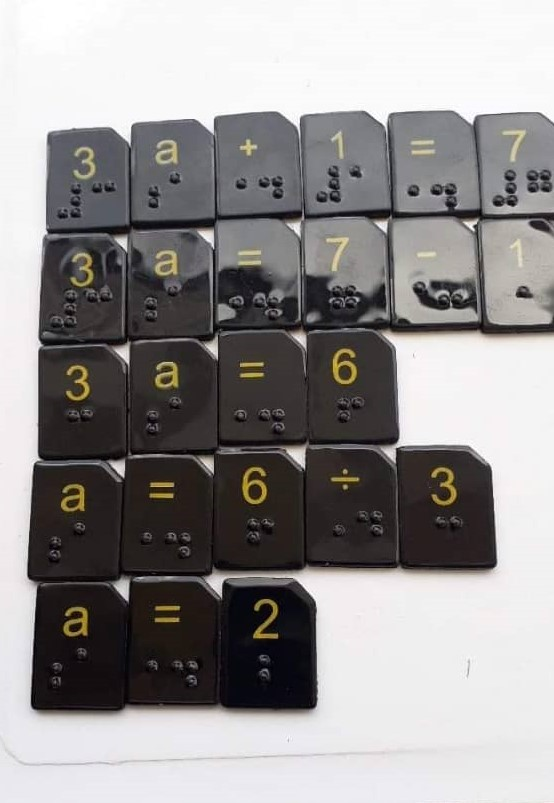
\includegraphics[width=0.55\linewidth]{images/fig1.jpg}
    \caption{Sample mathematic calculation with tiles and board}
\end{figure}

2. \textbf{STEM Kit\textcopyright{} Diagrams: }Below are samples of the STEM Kit\textcopyright{} diagrams. The diagrams depend on the classroom level of the BVI and the subject/topic to be taught. The diagrams are embossed so BVI can feel the diagram with their fingers and the teachers can see the prints. There are so many ways teachers can use the diagrams. They are presented with print and braille labels. Some are without labels, but we have individual labels having both print and braille labels. The teachers were taught different ways of using the diagrams to achieve effective teaching and learning. Below are examples:  

\begin{figure}[h]
    \centering
    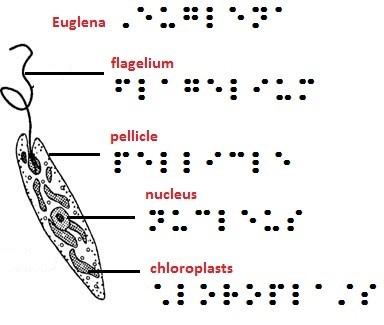
\includegraphics[width=1\linewidth]{images/fig2.jpg}
    \caption{Tactile diagram of Euglena a microscopic organism.}
\end{figure}

Euglena is one of the topics in basic science taught in secondary school. The braille and print labels are linked to the structure.

\begin{figure}[h]
    \centering
    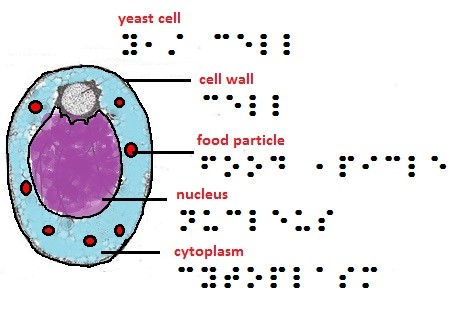
\includegraphics[width=1\linewidth]{images/fig3.jpg}
    \caption{Tactile Diagram of a yeast cell. A topic in secondary school basic science}
\end{figure}
\begin{figure}[h]
    \centering
    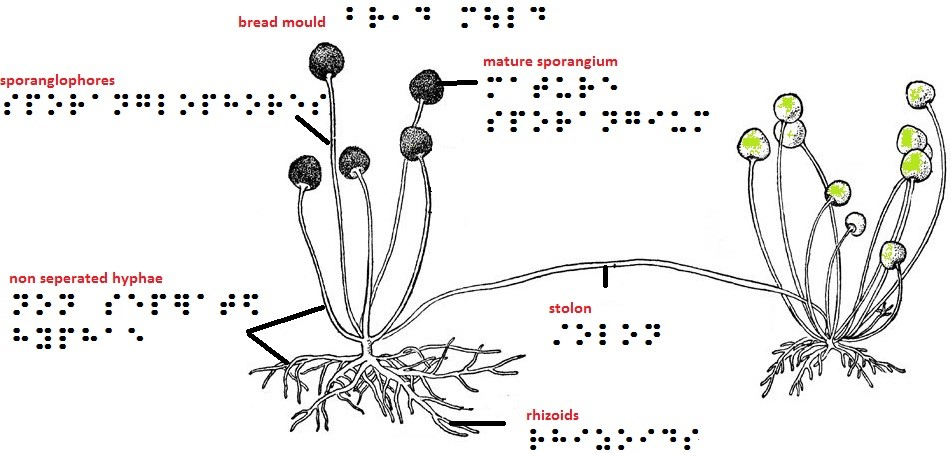
\includegraphics[width=1\linewidth]{images/fig4.jpg}
    \caption{Tactile Diagram of the bread mould. A topic in secondary school basic science}
\end{figure}

The Kit is often packaged together with some other resources to achieve full inclusion, such as:

\begin{enumerate}
    \item The Talking LabQuest
    \item Maths Talk Software
    \item Tactile Mathematical instruments
    \item Tactile adapted graph Sheets pack
\end{enumerate}

Below are brief explanations on these items.

1. \textbf{Talking LabQuest and Sensors:} This equipment (figure 5) allows the BVI to individually perform science experiment and or participate in group work with the sighted group mates. There are over 70 sensors. The sensor to be used depends on the experiment in question.

\begin{figure}[h]
    \centering
    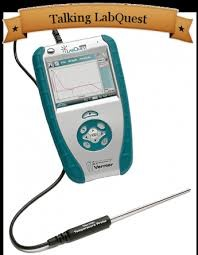
\includegraphics[width=0.6\linewidth]{images/fig5.jpg}
    \caption{A picture of the talking LabQuest connected to a temperature probe}
\end{figure}

2. \textbf{Maths Talk Software:} This is developed in Texas USA. The software allows students to use voice command to input many aspects of mathematics into the computer. It offers an easy way of examining students in calculations and some other aspects of the curriculum. The students can review workings upward and backward and answers can be reviewed before sending the documents to the printer. This allows the BVI to have feedback on their work same time with the sighted students. Figure 6 shows a screenshot of a sample calculation.

\begin{figure}[h]
    \centering
    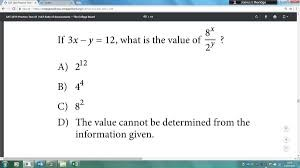
\includegraphics[width=1\linewidth]{images/fig6.jpg}
    \caption{Screenshot of a sample calculation with MathsTalk}
\end{figure}

3. \textbf{Tactile Mathematical instruments and Boards: }There are different rulers with braille markings or with tactile markings, which can be used by BVI in ways similar to the sighted or it could be use with limited adaptations

4. \textbf{Adapted graph Sheets: }Different graph sheets has been designed over time by different organisations and different methodologies of using the graph are demonstrated by each designer. In anycase, the graph sheet has tactile markings large enough to be felt and use by the BVI.

\section*{METHODOLOGY}
The whole research from which this report was taken adopted a multi approach research methodology. However, this part adopted case study approach in the evaluation of the tactile diagrams in the STEM Kit\textcopyright{}. Data were collected with:

\begin{itemize}
    \item Classroom observations
    \item Teachers  and Students interview
\end{itemize}

Two Inclusive secondary Schools were involved in intervention in the research while Basic Science and Technology Lessons were observed. The demographic of participants is shown in table I and II below:

\newcolumntype{P}[1]{>{\RaggedRight\arraybackslash}p{#1}}
\begin{table*}[!t]
\caption{Demographics of Students Participants}
\begin{tabular}{|l|l|l|l|l|}
\hline
& \textbf{Control }I & \textbf{Control II} & \textbf{Intervention I} & \textbf{Intervention II} \\ \hline
Students gender: & & & & \\
Male & 16 & 12 & 14 & 12 \\
Female & 06 & 08 & 08 & 13 \\ \hline
Age & & & & \\
10-13 & 12 & 07 & 10 & 11 \\
14-16 & 10 & 12 & 12 & 13 \\
17-19 & & 01 & & 01 \\ \hline
Education level: & & & & \\
Junior secondary II & 2 & 3 & 2 & 3 \\
Junior secondary III & 2 & 2 & 3 & 3 \\ \hline
Condition of visual impairment & \multicolumn{4}{l|}{BVI who are braille readers are involved in the study. They cannot read print} \\ \hline
\end{tabular}
\end{table*}

\begin{table*}[!t]
\caption{Demographics of Teacher Participants}
\begin{tabular}{|l|l|l|l|l|}
\hline
& \textbf{Control I} & \textbf{Control II} & \textbf{Intervention I} & \textbf{Intervention II} \\ \hline
Teachers gender: & & & & \\
Male & 2 & 3 & 0 & 1 \\
Female & 2 & 1 & 4 & 3 \\ \hline
Teachers Qualifications: & & & & \\ 
BCE & 3 & 2 & 2 & 3 \\ 
BSc & 1 & 2 & 2 & 2 \\ \hline
Years of Experience: & \multicolumn{4}{l|}{5 years Minimum teaching experience} \\ \hline
Specialist Knowledge & \multicolumn{4}{l|}{Teachers with no special education qualification are involved} \\ \hline
\end{tabular}
\end{table*}

This paper focused on three aspects:

Participation of the BVI in the lessons
 
Performance of the BVI specifically on the use of the diagrams

Peer learning among BVI and sighted classmates

The differences among participants’ genders and qualification are not the focus of this paper. The class was generally observed, and the participants’ interview responses are also considered generally.

\section*{PROCEDURE}
BVI in intervention schools were trained to interpret tactile diagrams. Tactile diagrams needed for the topics were produced and made available to intervention schools. Research assistant were also trained and coordinated to agree on what to record as important. The teachers presented the tactile diagrams the same time sighted have access to the printed diagrams. This was done for a whole term and the research assistants observe the classroom teachings during the teaching of basic science. Interviews were conducted with the teachers and the students separately. The research assistants recorded audio and audio-visuals and each day he shows the students the transcripts of the classroom observation and little adjustment proposed were implemented. The number of times a BVI make major act or contribution in relation to the use of the tactile diagrams is counted averaged and plotted in figure 7.  

\section*{FINDINGS}

\begin{figure}[!h]
    \centering
    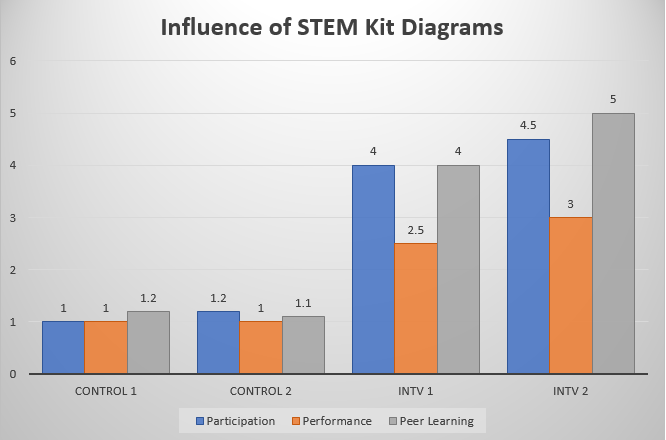
\includegraphics[width=1\linewidth]{images/fig7.png}
    \caption{A Stacked Bar Chart showing observed influence of STEM Kit\textcopyright{} diagrams on participation, performance and peer learning}
\end{figure}

\section*{DISCUSSION OF OBSERVATIONS}

The participation of BVI in the intervention classrooms improved tremendously to 4.0 and 4.5 as opposed to 1.0 and 1.2 in the control classrooms. Instead of total or partial passive attitude often exhibited the BVI contributed to the lessons, asked questions and answered questions. They participated more during the lessons taught with the STEM Kit\textcopyright{} tactile diagrams. BVI were more active during the lessons Similarly, their performance though, least affected improved from 1 in control classrooms to 2.5 and 3.0 in intervention classrooms. They were able to do what they are unable to do before. In the same way, the peer interaction and learning differs greatly from 1.1 and 1.2 in control classrooms to 4.0 and 5.0 in intervention classrooms.

\section*{SUMMARY FROM TEACHERS INTERVIEWS}

The teachers mentioned that the BVI accessed the diagrams and affirmed that their participation was increased. They were able to describe the diagrams and effectively identified the labels on the diagrams.  There was also improved peer learning, more interactions between them and their sighted classmates and these were mentioned by all teachers in the intervention schools. Improved Peer tutoring/in-teraction among BVI and sighted students occurred. Outside the teaching periods BVI and sighted students are seen exploring sample tactile diagrams.

\section*{SUMMARY FROM STUDENTS INTERVIEWS}

The BVI students expressed that they understood the topics better than when the diagrams are omitted for them. They wish all diagrams in all subjects are provided for them. They expressed that using the diagrams was the best thing that has ever happened in the school. All these expressions show that the tactile diagrams had a great impact on their learning.
 

\section*{CONCLUSION}

The STEM Kit\textcopyright{} diagrams from this study has removed communication gap between the BVI and their basic science teachers. They have equal access to diagrams in the topics taught unlike before. Their performance in basic science was least affected, this may be due to limited exploration of the diagram. Participation in classroom activities was improved greatly. Peer learning between SVI and sighted peers on the topics increased and the teacher and students wish to have diagrams in all subjects procured and distributed to schools by government. 


\section*{RECOMMENDATIONS}

The teacher trainers [Colleges and Universities] should prepare the teachers of visually impaired [TVI] adequately to be able to support teachers teaching STEM subjects in the primary and secondary schools where they are expected to work after the training. The situation where TVI are unable to support the teachers to access all aspects of the curriculum should change. Training them to adequately support mathematics and science teachers in inclusive schools will go a long way in making STEM subjects accessible to BVI. 

The government and Charity organisations are implored to make available adequate provision of resources and personnel in all-inclusive schools. They are implored to train teachers already on the field how to achieve inclusion of BVI in mathematics and sciences especially diagrams. It was recommended that the government or charity organisation can establish a central place for production of the tactile diagrams for all schools in the country and shared with people in other countries. Government should organise regular hands on workshop for BVI to build their confidence and equip them with necessary skills. This should be done with appropriate body that have the relevant knowledge. These would achieve adequate knowledge of tactile resources advanced by Beck-Winchatz .and Riccobono (2008)

The effect of student or teachers’ gender on the use of the tactile diagrams was not considered in this paper. It is recommended that further research be carried out to determine if they are influenced differently. STEM Kit diagrams use in other subjects should also be evaluated and possibly in the senior secondary school science subjects to determine its influence on the subjects. 

\end{large}
\clearpage
\section*{REFERENCES}\par 

\leftskip 0.25in
\parindent -0.25in 

Abilu, R. A. (2012) ‘Teaching Science and Mathematics to Learners with visual impairment in Nigeria: a perspective’ \textit{The Journal of Advocacy and Rehabilitation in Special Education (JARSE)} 11(1):78-82.

Adelakun, S. A. (2020) \textit{Making Mathematics and Science Accessible to the Blind}. LAP LAMBERT Academic Publishing

Adelakun, S. A (2013) ‘Inspirations from Scientists and Engineers Who Are Blind and Visually Impaired - Lessons to Initiate New Direction for Science Education of Blind Students in Nigeria’ \textit{Conference proceedings. International Conference new perspectives in science education} ISBN code (978-88-6292-351-4) Libreriauniversitaria.it. Edizioni,

Adelakun, S. A. (1994) ‘Effect of using adapted materials in teaching science to the visually impaired’ \textit{Journal of issues in Special Education} 2(2) 105-109.

Azanor, V. O. (2014) ‘A critic of inclusive educational programme in Nigeria JISSE’ 13 (1) \url{http://www.fcesjisse.edu.ng/ArticleDetails.aspx?id=36001} Accessed on 21 May, 2015

Beck-Winchatz, B.and Riccobono, M. A. (2008) ‘Advancing Participation of Blind Students in Science, Technology, Engineering, and Mathematics’ \textit{Advances in Space Research} 42:1855-1858.

Coville, M. G. (1932) ‘Content of a Course in General Science: Adapted for use with the Blind’ in Proceedings of \textit{31st Biennial Convention of the American Association of Instructors of the Blind} pp 773-775

Cryer, H. (2013) \textit{Teaching STEM Subjects to Blind and Partially Sighted students: literature review and resources} Birmingham: RNIB Centre for Accessible Information (CAI).

Cryer, H. and Gunn, D. (2008) \textit{Exploring Tactile Graphics} Birmingham: RNIB Centre for Accessible Information.

Eichenberger, R. J. (1974) ‘Teaching Science to the Blind Student’ \textit{Science Teacher} 41(9): 53-54.

Fraser, W. J. and Maguvhe, M. O. (2008) ‘Teaching Life Sciences to Blind and Visually Impaired Learners \textit{Journal of Biological Education} 42(2), 84-89.

Lewis, S. and Allman, C. B (2014) ‘Learning, Development and Children with Visual Impairments: The Evolution of Skills’ in C. B. Allman. and S. Lewis (Eds) \textit{ECC Essentials: Teaching the Expanded Core Curriculum to Students with Visual Impairments} New York: AFB Press:3-14.

Norman, K.,Caseau, D. and Stefanich, G. P. (1998) ‘Teaching Students with Disabilities in Inclusive Science Classrooms: Survey Results’ \textit{Science Education} 82: 127-146.

Sahin, M. and Yorek, N. (2009) ‘Teaching Science to Visually Impaired Students: a small-scale qualitative study’ \textit{US-China Education Review} 6 (4):19-26.

Wild, T., Hilson, M. and Hobson, S. (2013) ‘Conceptual Understanding of Sound by Elementary Students with Visual Impairments’ \textit{Journal of Visual Impairment and Blindness} 107 (2):107-116.

\end{document}